%----------------------------------------------------------------------------
\chapter{Jegyzőkönyv}
%----------------------------------------------------------------------------

%----------------------------------------------------------------------------
\section{Első feladat}
%----------------------------------------------------------------------------
\begin{figure}[!ht]
	\centering
	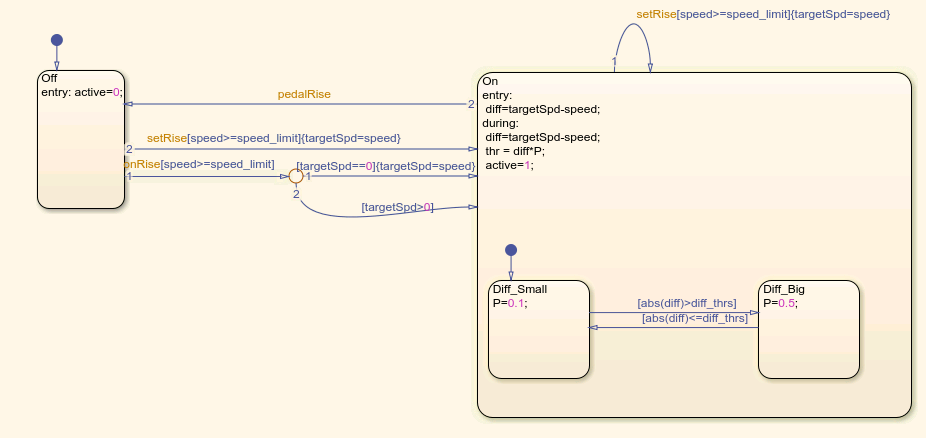
\includegraphics[width=120mm,keepaspectratio]{figures/2m04/f2_chart_2.png}
	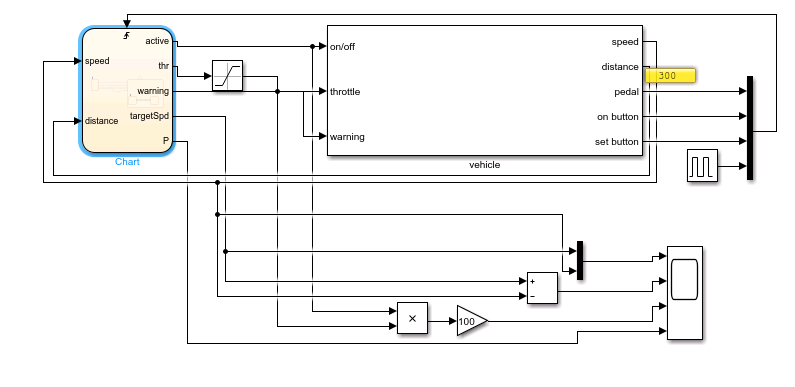
\includegraphics[width=120mm,keepaspectratio]{figures/2m04/f2_model_2.png}
	\caption{Az egyszerű tempomat modellje}
	\label{fig:chart1}
\end{figure}
Az első feladat megoldása során egy tempomatot implementáltam \textit{Stateflow} környezetben. A megvalósított rendszer és a benne található StateChart a \figref{chart1}~ábrán látható. A laboratórium során használt előre megírt Simulink modell z \textit{on/off} bemenetére 0 vagy 1 értéket vár, attól függően, hogy a tempomat aktív-e, ehhez hasonlóan a warning input a harmadik feladatban megvalósítandó jelzés állapotát várja. A kívánt gázpedálállást a \textit{throttle} bemeneten tudjuk egy 0 és 1 közötti értékként megadni a rendszernek. Kimenetként az aktuális sebesség, a jármű előtti akadály távolsága, valamint a nyomógombok és a pedál lenyomásának detektálására szolgáló jelek találhatóak.


A rendszerbe egy $T=0.1s$ periódusidejű pulzusgenerátort tettem, mely felfutó élre triggereli a \textit{StateChart} modellt. Ezen kívül az állapotgép "gázpedál-állás" kimenetét beszaturáltam 0 és 1 közé, hogy ne kaphasson a modell valótlan értéket. A könnyebb fejlesztés érdekében a sebességeket, azok különbségét, a kiadott gázpedál-állást, valamint a használt P erősítést is egy oszcilloszkópon jelenítettem meg, melyet a végleges modellnél kitöröltem.

Az állapotgép az \textit{Off} állapottal indul, ilyenkor a tempomat ki van kapcsolva. Ebből az állapotból az ON vagy a SET gomb megnyomásával lehet a tempomatot bekapcsolt állapotba helyezni. A SET gomb megnyomása esetén -akár bekapcsolt állapotban történő ismételt nyomásra is - a rendszer az aktuális sebességet veszi követendő referencia sebességnek. Az ON gomb esetén, ha már volt tárolt sebesség, akkor azt kezdi el használni.

A P-szabályzó figyelembe veszi a különbséget az aktuális és a követendő sebesség között, ez alapján állítja a gyorsítás értékét.

A \figref{scope1}~ábrán ennek az egyszerű modellnek a tesztelése látható, mely során egy kézi gyorsítás után a tempomatot bekapcsoltuk, az pedig követte a referenciasebességet. Mivel ez a rendszer első bekapcsolása volt, a kis hibajel miatt a a P értéke is kicsi maradt. 

\begin{figure}[!ht]
\centering
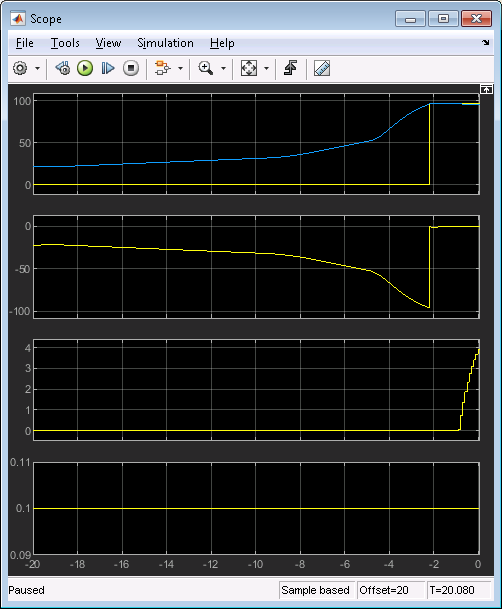
\includegraphics[width=110mm,keepaspectratio]{figures/2m04/f2_scope_2.png}
\caption{Az egyszerű tempomat tesztelése}
\label{fig:scope1}
\end{figure}

\newpage
%----------------------------------------------------------------------------
\section{Második feladat}
%----------------------------------------------------------------------------
\begin{figure}[!ht]
	\centering
	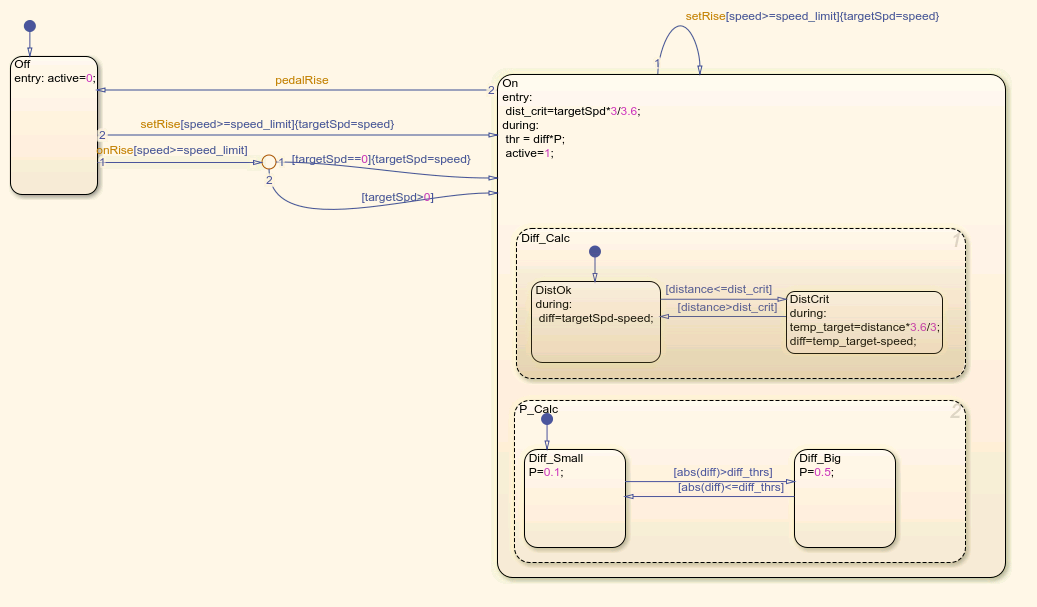
\includegraphics[width=120mm,keepaspectratio]{figures/2m04/f2_chart_3.png}
%	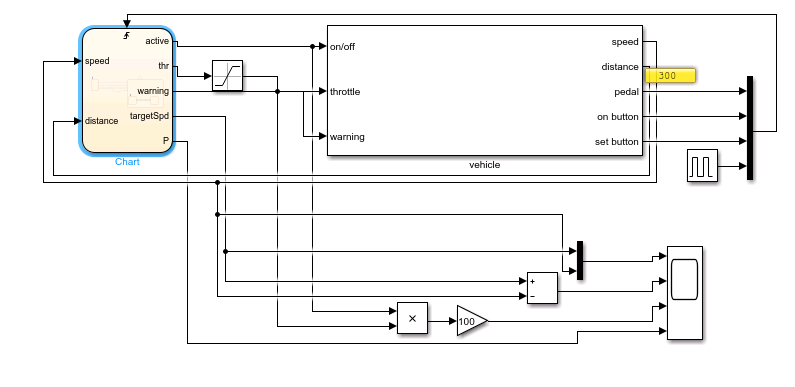
\includegraphics[width=120mm,keepaspectratio]{figures/2m04/f2_model_2.png}
	\caption{Az adaptív tempomat állapotgépe}
	\label{fig:chart2}
\end{figure}

Az adaptív tempomat megvalósítása során a távolságérzékelőből jövő \textit{distance} jelet kellett felhasználni. A beállított referencia sebesség alapján számolható egy kritikus úthossz (a modellben \textit{dist\_crit} nevű változó), mely megadja, hogy az adott sebességgel hány métert tesz meg a jármű a feladatkiírásban szereplő 3 másodperc alatt. A \figref{chart2}~ábrán látható a kibővített állapotgép, mely a \textit{DistOK} állapotban marad, egészen addig, amíg a kritikus úthossz alá nem csökken a \textit{distance} jel. Ekkor a \textit{DistCrit} állapotban a rendszer egy új refrencia sebességet számol a mért távolság alapján, hogy az adaptívan követni tudja a jármű előtti akadályt, például egy másik járművet. Mivel a tempomat bekapcsolt állapota mellett mind a távolság, mind a P erősítés számolását meg kell valósítani, így azokat \textit{AND} kompozícióval valósítottam meg.

A modell tesztelésére szolgáló mérés a \figref{scope2}~ábrán látható. A kék jel az autó tényleges sebessége, a sárga jelek sorban a sofőr által beállított referencia sebesség, előző kettő különbsége, a kiadott gázpedálállás jel \%-os formában, valamint a távolságérzékelőből jövő jel. Jól látszik, hogy a mérés szüneteltetését előtt kb. 30 másodperccel kritikusan közel jött egy akadály a jármű előtt, ezért a tempomat azonnal elvette a pedálnyomást. Nagyjából -19s környékén az autó annyira visszalassult, hogy a követendő távolság tartásához ismét növelni kell a gázpedálnyomás értékét, melyet a rendszer meg is tesz. A mérés vége előtt 10 másodperccel az akadály eltűnt a jármű előtt, így az visszaáll az eredetileg beállított referencia sebesség követésére.

A mérés során jól látható a P-szabályzó hátránya, a beállított sebességet konstans leköveti, ám a maradandó hiba miatt azt sosem éri el.

\begin{figure}[!ht]
	\centering
	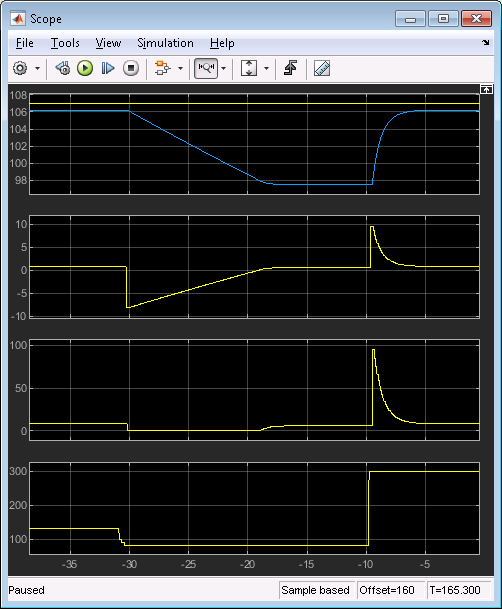
\includegraphics[width=110mm,keepaspectratio]{figures/2m04/f2_scope_3.png}
	\caption{Az adaptív tempomat tesztelése}
	\label{fig:scope2}
\end{figure}




\newpage
asdasdfasdf
\newpage
asdasdfasdf
\newpage
%----------------------------------------------------------------------------
\section{A labor témája}
%----------------------------------------------------------------------------
A mérés során egy sorompó irányítását terveztük meg, melyet a diszkrét eseményű rendszerek felügyeleti irányításával valósítottunk meg. A modellt és annak specifikációit a Supremica programban alkottuk meg, majd azt a Matlab Stateflow bővítményének segítségével teszteltük.


%----------------------------------------------------------------------------
\section{Szabályozandó szakasz megtervezése}
%----------------------------------------------------------------------------
A sorompót mozgató motor modellje a \figref{Motor}~ábrán látható. Három állapota lehet, vagy fel-, vagy lemozgatja a sorompó rudat, vagy egy helyben tartja azt. 

\begin{figure}
	\centering
	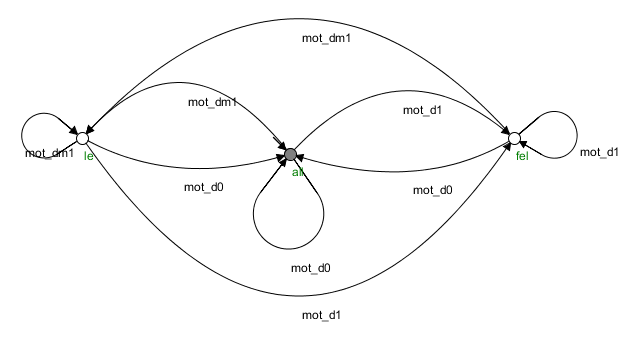
\includegraphics[width=110mm,keepaspectratio]{figures/2m03/b_motor.png}
	\caption{A sorompó rúd mozgató motor modellje}
	\label{fig:Motor}
\end{figure}
Ezen állapotok között a következő eseményekkel lehet váltani:
\begin{itemize}
	\item \textbf{mot\_d1} - Sorompó felfelé indítása
	\item \textbf{mot\_dm1} - Sorompó lefelé indítása
	\item \textbf{mot\_d0} - Sorompó megállítása
\end{itemize}
Mint látható, ezen modell megengedi, hogy a mozgás közben ismételten ráindítsunk a motorra, álló helyzetben ismét leállítsuk vagy akár ellentétes irányú ráindítás is lehetséges, mely a motor élettartamát jelentősen csökkentené. Ezen jelenségek letiltása miatt egy specifikációt vezettünk be, mely a \figref{SpecMot}~ábrán látható.

\begin{figure}
	\centering
	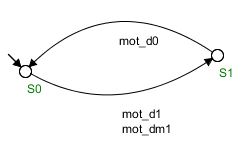
\includegraphics[keepaspectratio]{figures/2m03/b_spec_motor.png}
	\caption{A mozgató motor specifikációja}
	\label{fig:SpecMot}
\end{figure}
A Supremica \textit{Analyzer} fülén az eddig megvalósított automaták szinkron szorzatát a \textit{Synchronize} paranccsal valósítottuk meg, az így készült modell (továbbiakban \textit{sup\_mot}) -mely már megfelel a specifikációnak- a \figref{SupMot}~ábrán látható.
\begin{figure}
	\centering
	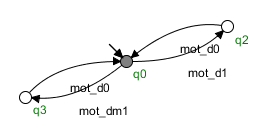
\includegraphics[keepaspectratio]{figures/2m03/b_supmot.png}
	\caption{A mozgató motor végleges modellje}
	\label{fig:SupMot}
\end{figure}


\newpage
%----------------------------------------------------------------------------
\section{A végálláskapcsoló és fizikai korlátok}
%----------------------------------------------------------------------------
A motor helyes vezérléséhez szükségünk lesz egy-egy végálláskapcsolóra, mely a legfelső (\textit{top\_}), illetve legalsó (\textit{bottom\_}) helyzet elérését jelzik, vagyis a motor megállítására figyelmeztetnek. Eddig a modellben csak általunk irányítható eseményeket vettünk fel, ám a végálláskapcsoló jelzésének idejét nem tudjuk kontrollálni, ezt külön meg kell jelölnünk a Supremicában. Mindkét kapcsoló jelének fel, illetve lefutó élére következik be esemény, ezeket a \textit{rise} és \textit{fall} címkével jeleztük. A végálláskapcsolókhoz tartozó automata (\figref{Limit}~ábra) kezdeti állapota az, hogy a sorompó az alsó végállásban van. További állapotok, ha két végállás között valahol félúton, vagy a felső végállásban van a sorompó rúd.
\begin{figure}
	\centering
	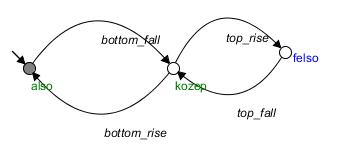
\includegraphics[keepaspectratio]{figures/2m03/b2_limit.png}
	\caption{A végálláskapcsolók modellje}
	\label{fig:Limit}
\end{figure}
Mivel nem irányítható eseményeket terveztünk a rendszerbe, így azok jelenleg bármikor bekövetkezhetnek, ám helyes működés esetén ezen eseményeknek fizikai korlátai vannak. Feltételezhetjük, hogy az alsó végálláskapcsoló jelzésének lefutó éle, és a felső kapcsoló jelzésének felfutó éle csak a sorompó felfelé mozgása közben következhet be. Ehhez hasonlóan a \textit{top\_fall}, illetve a \textit{bottom\_rise} esemény csak lefelé mozgás közben történhet. Ezeket a fizikai korlátokat is felvittük a programba, melyek a \figref{Constraints}~ábrán láthatóak.

\begin{figure}
	\centering
	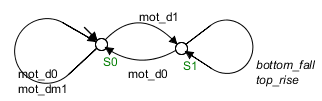
\includegraphics[keepaspectratio]{figures/2m03/b2_constr1.png}	
	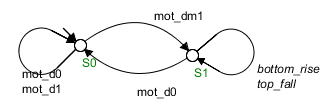
\includegraphics[keepaspectratio]{figures/2m03/b2_constr2.png}
	\caption{A fizikai korlátok modelljei}
	\label{fig:Constraints}
\end{figure}

Az előző pontban taglalt \textit{sup\_mot}, valamint az ebben a pontban megvalósított automaták szinkron szorzatát véve elkészítettük a \textit{barrier} modellt, mely a sorompó mozgatását megvalósító funkciók összesített modellje. Ennek állapotgráfja látható a \figref{Barrier}~ábrán.

\begin{figure}
	\centering
	\includegraphics[trim = 10mm 55mm 50mm 10mm,clip,width=140mm,keepaspectratio]{figures/2m03/barrier2.pdf}
	\caption{A sorompó mozgatását megvalósító funkciók állapotgráfja}
	\label{fig:Barrier}
\end{figure}




%----------------------------------------------------------------------------
\section{Az infraérzékelő és a távirányító}
%----------------------------------------------------------------------------
A sorompó akkor működik jól, ha az nem záródik rá és nem tesz kárt az ügyfél gépjárművében. Ennek megakadályozására infrasugaras érzékelőt használunk, melyet a rendszerbe kell integrálnunk. Továbbá az ügyfél szeretné távirányítóval nyithatóvá tenni a sorompót. E két rendszer modellje látható a \figref{InfraRemote}~ábrán, melyen az infra jel felfutó éle jelzi az akadály megjelenését, illetve a lefutó éle annak eltűnését. A távirányító szempontjából elég nekünk a gomb megnyomását érzékelnünk. Ezen események ismét általunk kontrollálhatatlanok, ezeket jelezni kell a programnak. 

\begin{figure}
	\centering
	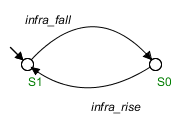
\includegraphics[keepaspectratio]{figures/2m03/b2_infra.png}	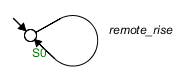
\includegraphics[keepaspectratio]{figures/2m03/b_remote.png}
	\caption{Az infraérzékelő és a távirányító modelljei}
	\label{fig:InfraRemote}
\end{figure}

Az eddig meglévő \textit{barrier}, illetve az újonnan megvalósított két modellt ismét \textit{szinkronizáljuk} a Supremica segítségével, továbbiakban ez lesz a plant, mely a \figref{Plant}~ábrán látható.

\begin{figure}
	\centering
	\includegraphics[trim = 15mm 70mm 50mm 10mm,clip,width=140mm,keepaspectratio]{figures/2m03/plant.pdf}
	\caption{A teljes rendszer működését megvalósító állapotgép}
	\label{fig:Plant}
\end{figure}

\newpage
%----------------------------------------------------------------------------
\section{Specifikációk}
%----------------------------------------------------------------------------
Az eddigi rendszer képes a működésre, ám nem feltétlenül a helyes, kontrollált módon. Ehhez ismét specifikációkat kell bevezetnünk, melyek a következők:
\begin{itemize}
	\item Ha visszatért az alaphelyzetben egészen addig nem mozoghat, amíg nem jön új gombnyomás.
	\item Ne indítsuk el a motort felfelé, ha már a felső végállásban vagyunk.
	\item Ha már elindultunk felfelé, akkor ne álljunk meg, amíg nem értük el a felső véghelyzetet.
	\item Csak akkor indulhatunk lefelé, ha a felső véghelyzetben vagyunk.
	\item Ha van akadály, akkor nem indulhatunk lefelé.
	\item Infra jelzésre, a távirányító megnyomására vagy az alsó végállás elérése esetén álljunk meg a lefelé menettel.
\end{itemize}

\begin{figure}
	\centering
	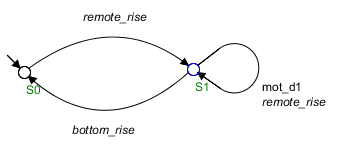
\includegraphics[keepaspectratio]{figures/2m03/b_spec1.png}
	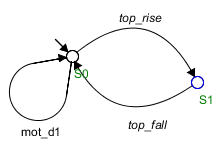
\includegraphics[keepaspectratio]{figures/2m03/b_spec2.png}
	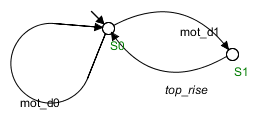
\includegraphics[keepaspectratio]{figures/2m03/b_spec3.png}
	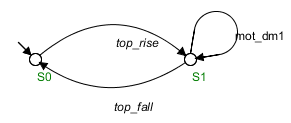
\includegraphics[keepaspectratio]{figures/2m03/b_spec4.png}
	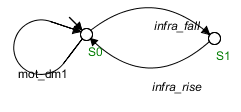
\includegraphics[keepaspectratio]{figures/2m03/b_spec5.png}
	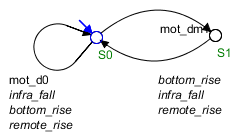
\includegraphics[keepaspectratio]{figures/2m03/b_spec6.png}
	\caption{A definiált specifikációk modelljei}
	\label{fig:SpecAll}
\end{figure}

A megvalósított specifikációk a \figref{SpecAll}~ábrán láthatóak, melyek létrehozásában segített a \textit{Controllability Check} funkció, mely ellenőrzi és figyelmeztet az esetleges kontrollálhatatlan események bekövetkeztének lehetőségére.

A teljes rendszer és a megvalósított specifikációk kijelölése után a \textit{Synthesize} menüponttal megterveztük a szabályzót. Az elkészült rendszer zárt köre a \figref{ClosedLoop}~ábrán látható.

\begin{figure}
	\centering
	\includegraphics[trim = 0mm 55mm 260mm 0mm,clip,width=140mm,keepaspectratio]{figures/2m03/closedloop.pdf}
	\caption{A sorompó mozgatását megvalósító funkciók állapotgráfja}
	\label{fig:ClosedLoop}
\end{figure}

%----------------------------------------------------------------------------
\section{Szimuláció}
%----------------------------------------------------------------------------
A megtervezett rendszert a Supremicából XML formátumba exportáltuk, melyet az előre megírt \textit{sup2sim script} segítségével Matlab Simulink modellé tudtuk alakítani. Ezután a szimulációt megvalósító modellel összekötöttük a megfelelő jeleket egy multiplexer segítségével (\figref{SimModel}~ábra) és elindítottuk a szimulációt. A grafikus felületen lehetőségünk volt a nyomógomb nyomását, illetve akadály érzékelését imitálni.
A \figref{Sim}~ábrán a következő események láthatóak:
\begin{itemize}
	\item A sorompó alaphelyzete. Látható, hogy az alsó végálláskapcsoló jelez.
	\item A gombnyomás hatására elindul a sorompó felfele.
	\item A rendszer akadályt érzékel, ezért a sorompót a felső végállásban tartja.
	\item Az akadály eltűnése után a sorompó lefelé mozog.
\end{itemize}

A szabályzó a szimulációk során az elvártaknak megfelelően működött.



\begin{figure}
	\centering
	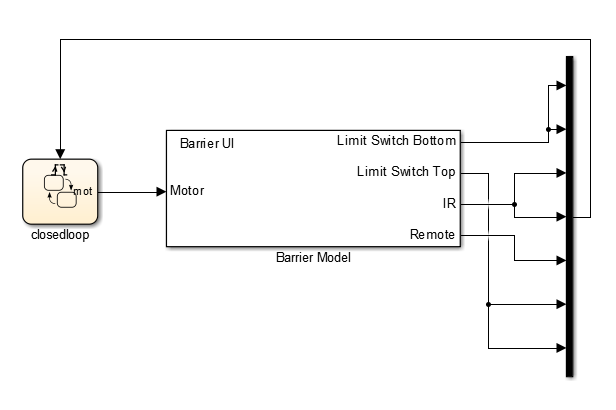
\includegraphics[keepaspectratio]{figures/2m03/b_sim.png}
	\caption{A szimuláció modellje}
	\label{fig:SimModel}
\end{figure}


\begin{figure}
\centering
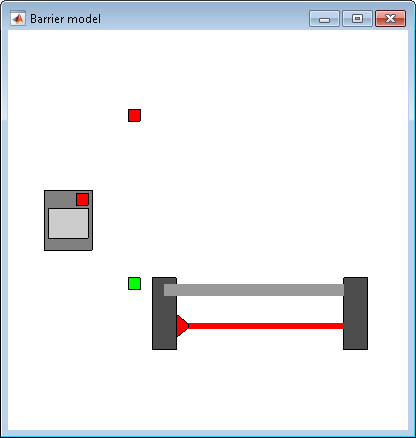
\includegraphics[width=70mm, keepaspectratio]{figures/2m03/b2_sim1.png}\vspace{2mm}
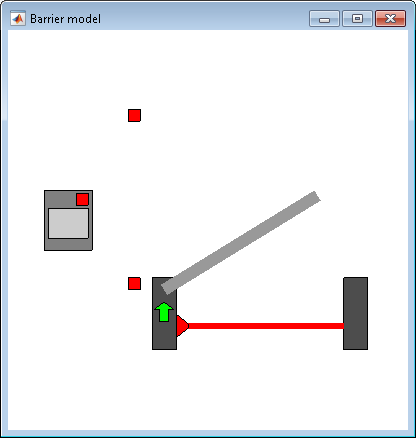
\includegraphics[width=70mm, keepaspectratio]{figures/2m03/b2_sim2.png}\hspace{2mm}
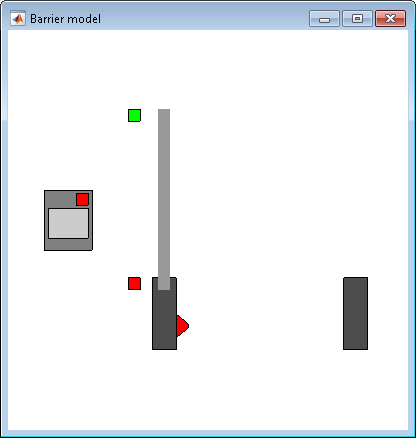
\includegraphics[width=70mm, keepaspectratio]{figures/2m03/b2_sim3.png}\vspace{2mm}
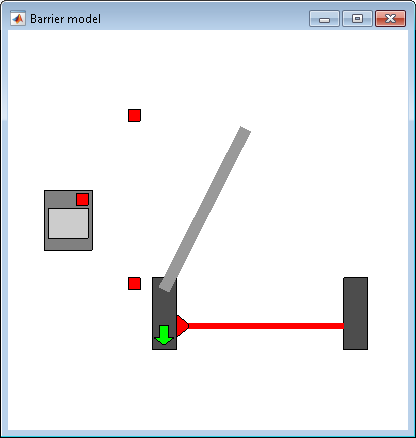
\includegraphics[width=70mm, keepaspectratio]{figures/2m03/b2_sim4.png}
\caption{A szimuláció}
\label{fig:Sim}
\end{figure}